% draft of Section 2.1 (Illustrative Example).  Not part of the manuscript.
% toy: demand 1 or 3, capacity 3, advance orders up to 2 at price 30, later orders at price 30 plus rush cost 20 (site 1) or 90 (site 2),
%      opening cost 60 (site 1) or 67 (site 2), estimate 0.8, range 0.5 to 1.0.  check: toy_check_mean_v5.py
\documentclass[ijoc,dblanonrev]{informs4}
\RequirePackage{tgtermes}
\RequirePackage{newtxtext}
\RequirePackage{newtxmath}
\RequirePackage{bm}
\usepackage{booktabs}
\usepackage{caption}
\usepackage{subcaption}
\usepackage{tikz}
\OneAndAHalfSpacedXII
\EquationsNumberedThrough
\TheoremsNumberedThrough
\MANUSCRIPTNO{}
\begin{document}
\setcounter{section}{1}
\section{Problem Setting}
\subsection{Illustrative Example}
\label{subsec:example}

We illustrate with a stylized example that ambiguity in the truth and
ambiguity in the follower's belief cannot be treated separately. In this
example, the decision that is optimal under the leader's estimate remains
optimal when either the truth or the belief alone is misspecified, and it
becomes suboptimal when both are.

Consider a supplier (the leader) who opens one of two sites with a capacity of
three units, at a cost of 60 for site~1 and 67 for site~2, and a buyer (the
follower) whose demand $\xi$ is either low ($\xi = 1$) or high ($\xi = 3$).
Before the demand is realized, the follower places an advance order of
$h \in [0,2]$ units at a unit price of 30, which is paid regardless of the
demand. Once the demand is realized, he orders the shortfall $(\xi - h)^{+}$
at the same price and incurs an additional rush cost of $t$ per unit, where
$t = 20$ at site~1 and $t = 90$ at site~2. The leader is risk-neutral and
collects the price of every unit ordered, so that her revenue equals
$30\max\{h, \xi\}$.

Let $p$ and $\tilde p$ denote the probabilities of high demand under the truth
and under the follower's belief, respectively. The follower minimizes
$30h + (30 + t)\,\mathbb{E}^{\tilde p}[(\xi - h)^{+}]$ over $h \in [0,2]$,
which is piecewise linear in $h$. Under the pessimistic convention, his
advance order is $h = 2$ if $\tilde p > 30/(30 + t)$ and $h = 1$ otherwise,
and the threshold equals $0.6$ at site~1 and $0.25$ at site~2. The leader's
expected profit is therefore $30p$ at site~1 if $\tilde p > 0.6$, $60p - 30$
at site~1 if $\tilde p \le 0.6$, and $30p - 7$ at site~2 if $\tilde p > 0.25$.

\begin{table}[!h]
\begin{minipage}[t]{0.54\linewidth}
\centering
\captionof{table}{Leader's expected profit by site, truth $p$ and follower's belief $\tilde p$.}
\label{tab:toy}
\vspace{6pt}
\small
\begin{tabular}{@{}lccc@{}}
\toprule
 & \multicolumn{2}{c}{Site 1} & Site 2\\
\cmidrule(lr){2-3}\cmidrule(l){4-4}
 & $\tilde p > 0.6$ & $\tilde p \le 0.6$ & $\tilde p > 0.25$\\
\midrule
Advance order $h$ & 2 & 1 & 2\\
\midrule
Profit at $p = 0.8$ & 24 & 18 & 17\\
Profit at $p = 0.5$ & 15 & 0 & 8\\
Profit at general $p$ & $30p$ & $60p - 30$ & $30p - 7$\\
\bottomrule
\end{tabular}
\end{minipage}\hfill
\begin{minipage}[t]{0.43\linewidth}
\centering
\captionof{figure}{Leader's expected profit against the truth $p$.}
\label{fig:toy}
\vspace{2pt}
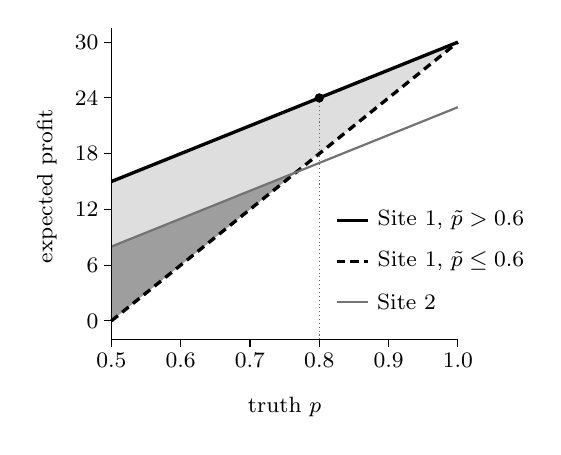
\begin{tikzpicture}[x=8.8cm, y=0.118cm, font=\footnotesize, >=stealth]
  % loss at site 1 when the follower does not order the second unit in advance
  \fill[black!13] (0.5,15) -- (1.0,30) -- (0.5,0) -- cycle;
  % truths at which site 2 is better when the belief is below the threshold
  \fill[black!38] (0.5,8) -- (0.7667,16) -- (0.5,0) -- cycle;
  % estimate
  \draw[densely dotted, black!60] (0.8,-2) -- (0.8,24);
  % the three profit lines
  \draw[very thick] (0.5,15) -- (1.0,30);
  \draw[very thick, densely dashed] (0.5,0) -- (1.0,30);
  \draw[thick, black!55] (0.5,8) -- (1.0,23);
  \fill (0.8,24) circle (1.7pt);
  % legend in the empty lower right corner
  \draw[very thick] (0.825,10.8) -- (0.87,10.8) node[right, inner sep=3pt] {Site 1, $\tilde p > 0.6$};
  \draw[very thick, densely dashed] (0.825,6.4) -- (0.87,6.4) node[right, inner sep=3pt] {Site 1, $\tilde p \le 0.6$};
  \draw[thick, black!55] (0.825,2.0) -- (0.87,2.0) node[right, inner sep=3pt, text=black] {Site 2};
  % axes and ticks
  \draw (0.5,-2) -- (1.0,-2); \draw (0.5,-2) -- (0.5,31.5);
  \foreach \v in {0.5,0.6,0.7,0.8,0.9,1.0} { \draw (\v,-2) -- (\v,-2.8) node[below, inner sep=2pt] {\v}; }
  \foreach \v in {0,6,12,18,24,30} { \draw (0.5,\v) -- (0.49,\v) node[left, inner sep=2pt] {$\v$}; }
  \node[below] at (0.75,-7.2) {truth $p$};
  \node[rotate=90, above] at (0.435,14.5) {expected profit};
\end{tikzpicture}

\vspace{-2pt}
{\footnotesize\textit{Note.} Light shading, loss of site~1 if $\tilde p \le 0.6$. Dark shading, site~2 outperforms site~1.\par}
\end{minipage}
\end{table}

Suppose that the leader's estimate of $p$ is $0.8$. If the follower shares
this estimate, site~1 is optimal with an expected profit of 24, compared with
17 for site~2 (Table~\ref{tab:toy}). Now let the truth and the belief each lie
within $0.3$ of the estimate. If only the truth is misspecified, the expected
profit decreases by at most 9 at either site, and site~1 remains optimal. If
only the belief is misspecified, the expected profit of site~1 decreases by 6
while that of site~2 is unaffected, and site~1 again remains optimal. If both
are misspecified, however, the expected profit of site~1 decreases by up to
24, which exceeds the sum of the two individual losses, and site~2 becomes
optimal with a worst-case expected profit of 8 compared with zero for site~1.

The loss is not additive because the advance order transfers the demand risk
of the second unit from the leader to the follower. When the belief falls
below the threshold, this risk reverts to the leader, and her expected loss
$30(1 - p)$ increases as the truth deteriorates (Figure~\ref{fig:toy}). At
site~2, the advance order is insensitive to the belief over the range
considered, at the expense of a lower profit under the estimate. The leader's
decision therefore affects not only her profit but also the sensitivity of
the follower's response to his belief.

The example has two implications for the ambiguity set. First, the set needs
to contain pairs of a truth and a belief, since the worst case is attained
when both deviate from the estimate. Second, such joint deviations are
plausible, since the follower forms his belief from the same data-generating
process. Section~2.3 introduces an ambiguity set with both properties.

\end{document}
